\documentclass[11pt,a4paper]{ivoa}
\input tthdefs
\input gitmeta

\title{Authentication for Non-Browser Clients in the VO}

% see ivoatexDoc for what group names to use here; use \ivoagroup[IG] for
% interest groups.
\ivoagroup{Distributed Services and Protocols}

\author{Patrick Dowler}
\author{Mark Taylor}
\author{Sara Bertocco}

\editor{Sara Bertocco}

% \previousversion[????URL????]{????Concise Document Label????}
\previousversion{This is the first public release}


\begin{document}
\begin{abstract}
Some, though not all, services in the Virtual Observatory are
restricted to users who have been authenticated and are authorized to use them.
This situation is far from unique to the VO,
and there is much industry-standard technology to manage authentication.
However, it largely assumes that authenticating clients,
often browser-based, understand how authentication is to be done
for a particular service.
This document addresses a problem apparently not covered
by existing standards, namely how a VO client can discover
authentication requirements and use the corresponding mechanisms
to supply user credentials
when pointed at a compliant VO service, without requiring out-of-band
information.
\end{abstract}


\section*{Acknowledgments}

\textcolor{red}{Editor's note: this section has to be
updated/rewritten. Authors who have someone to thank should
add here acknowledgments}
This document derives from discussions among the Grid and Web Services
working-group of IVOA. It is particularly informed by prototypes built
by Mark Taylor (University of Bristol) and Patrick Dowler
(Canadian Astronomy Data Centre).


\section*{Conformance-related definitions}

The words ``MUST'', ``SHALL'', ``SHOULD'', ``MAY'', ``RECOMMENDED'', and
``OPTIONAL'' (in upper or lower case) used in this document are to be
interpreted as described in IETF standard RFC2119 \citep{std:RFC2119}.

The \emph{Virtual Observatory (VO)} is a
general term for a collection of federated resources that can be used
to conduct astronomical research, education, and outreach.
The \href{https://www.ivoa.net}{International
Virtual Observatory Alliance (IVOA)} is a global
collaboration of separately funded projects to develop standards and
infrastructure that enable VO applications.


\section{Introduction}

Historically many services in the VO have operated primarily or
entirely in anonymous mode.
However authentication and in some cases authorization
are becoming increasingly required,
for instance to manage data rights and as an operational necessity for
auditing service usage in the era of science platforms.
% Some way to manage authentication for VO services is therefore necessary
% but not covered in all contexts by existing industry-standard machinery.

Where the client is browser-based
it is often possible to integrate information about the authentication
methods required with the web page or web application through which
it is accessed.
[is this true?  I don't understand browser-based authentication
or what makes it work all that well]

But a classic desktop VO client such as Aladin, TOPCAT or Python
typically interacts with VO services differently, in one of two
ways:
\begin{enumerate}
\item Search the registry for a service, then make VO-compliant
      requests to that service (e.g.\ TAP)
\item Be presented with a URL, then retrieve the data from that URL
      (e.g.\ DataLink)
\end{enumerate}
In the first, TAP-like, case additional information is available to the
client in the form of the Registry record for the service in question.
This could in principle contain metadata describing the authentication
method along with any required ancillary information such as
login endpoints.
Even in the TAP-like case in which only the TAP service URL is available
(for instance because the user has typed it in rather than acquired it
from a Registry search) the VOSI Capabilities endpoint can be reliably
located ({\tt /capabilities} is a sibling of {\tt sync} in TAP),
and relevant VOResource information could be retrived from the VOSI
Capabilities document.

However in the second, DataLink-like, case
there is no information about where to find a corresponding
registry record or VOSI document,
or even a guarantee or likelihood that such a record exists.
The URL in question may not even have come from a DataLink query,
it could simply be a pointer to a protected resource like a
FITS file or VOTable on a secured archive.
Such URLs may have been acquired from a VO query in the application
wishing to dereference them,
but they may equally be in a column of a VOTable transmitted by SAMP
or saved in an earlier session or from an unrelated application.
Then the only opportunity to acquire information about how to authenticate
is by examining the URL itself, or by communicating with the
service providing it.

HTTP Basic serves this need, but more modern/secure/flexible authentication
methods such as OAuth (surprisingly?) 

\subsection{Role within the VO Architecture}

\begin{figure}
\centering

% As of ivoatex 1.2, the architecture diagram is generated by ivoatex in
% SVG; copy ivoatex/archdiag-full.xml to role_diagram.xml and throw out
% all lines not relevant to your standard.
% Notes don't generally need this.  If you don't copy role_diagram.xml,
% you must remove role_diagram.pdf from SOURCES in the Makefile.

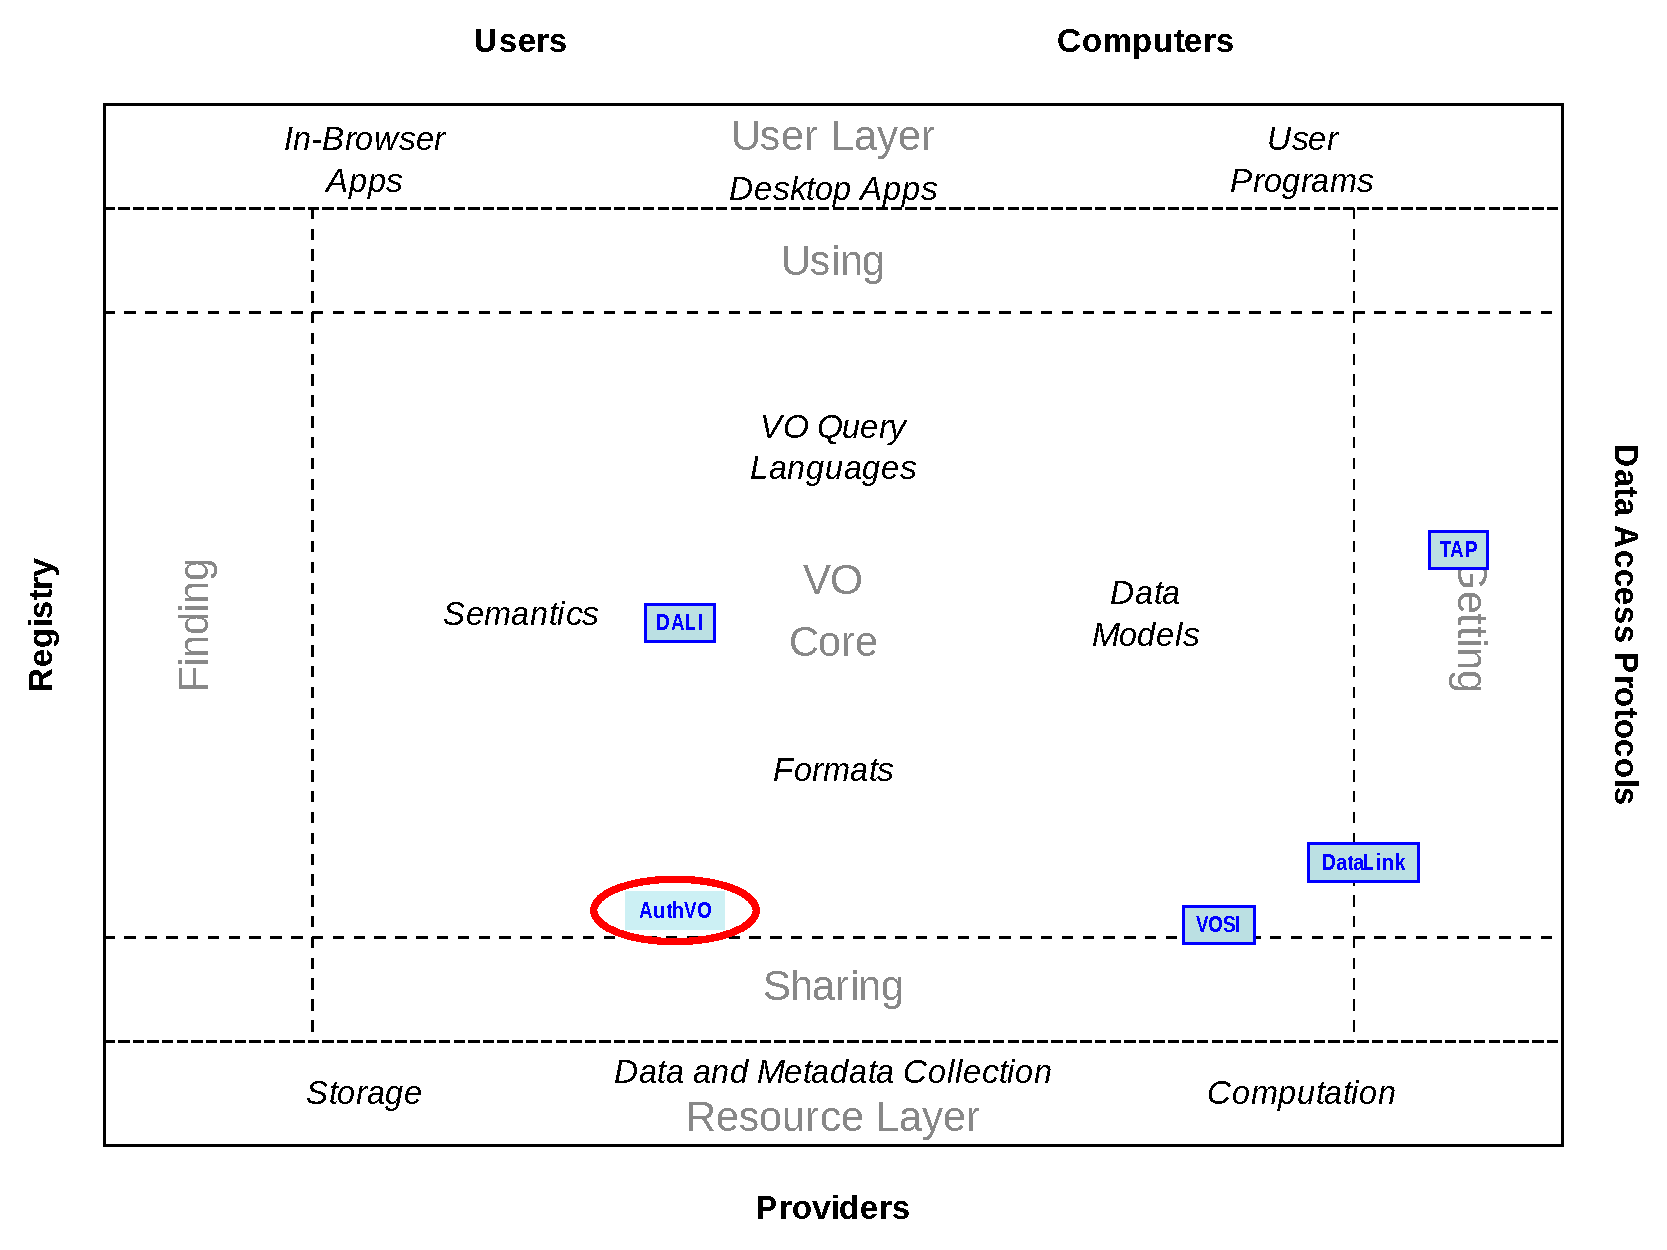
\includegraphics[width=0.9\textwidth]{role_diagram.pdf}
\caption{Architecture diagram for this document}
\label{fig:archdiag}
\end{figure}

Fig.~\ref{fig:archdiag} shows the role this document plays within the
IVOA architecture \citep{2021ivoa.spec.1101D}.

???? and so on, LaTeX as you know and love it. ????

\appendix
\section{Changes from Previous Versions}

No previous versions yet.
% these would be subsections "Changes from v. WD-..."
% Use itemize environments.


% NOTE: IVOA recommendations must be cited from docrepo rather than ivoabib
% (REC entries there are for legacy documents only)
\bibliography{ivoatex/ivoabib,ivoatex/docrepo}


\end{document}
